\documentclass[10pt,twocolumn]{article}
\usepackage[a4paper,top=0.60in,bottom=0.60in,left=0.60in,right=0.60in,columnsep=0.26in]{geometry}
\usepackage{amsmath,amssymb,amsfonts}
\usepackage{graphicx}
\usepackage{booktabs}
\usepackage{array}
\usepackage{enumitem}
\usepackage[font={footnotesize},labelfont=bf,skip=4pt]{caption}
\usepackage{titlesec}
\usepackage{xcolor}
\usepackage{microtype}
\usepackage[colorlinks=true,linkcolor=blue!60!black,citecolor=blue!60!black,urlcolor=blue!70!black]{hyperref}

\graphicspath{{figures/}{../results/runs/v4/figures/}{../experiments/}}

% Comfortable, breathable section and paragraph spacing
\titlespacing*{\section}{0pt}{8pt plus 2pt minus 1pt}{4pt plus 1pt}
\titlespacing*{\subsection}{0pt}{6pt plus 1pt minus 1pt}{2.5pt plus 1pt}
\titleformat{\section}{\normalfont\normalsize\bfseries}{\thesection.}{0.5em}{}
\titleformat{\subsection}{\normalfont\small\bfseries}{\thesubsection}{0.4em}{}

\setlength{\parindent}{0pt}
\setlength{\parskip}{3.5pt}
\setlength{\textfloatsep}{8pt plus 2pt minus 2pt}
\setlength{\floatsep}{6pt plus 2pt minus 1pt}
\setlength{\abovedisplayskip}{5pt plus 1pt minus 1pt}
\setlength{\belowdisplayskip}{5pt plus 1pt minus 1pt}
\setlist[itemize]{leftmargin=1.3em,itemsep=2pt,topsep=2pt,parsep=0pt}

\begin{document}
\fontsize{9.4pt}{11.4pt}\selectfont

\twocolumn[{%
\begin{@twocolumnfalse}
\begin{center}
    {\Large \textbf{FarmRL: Reinforcement Learning for Crop Input Management and Market Timing}}\\[6pt]
    {\normalsize \textbf{Harshita Vachhani} (B23EE1026) \quad and \quad \textbf{Aurindum Banerjee} (B23CS1006)}\\[3pt]
    {\small CSL3090: Artificial Intelligence (Assignment 2) $\cdot$ Indian Institute of Technology Jodhpur}\\
    {\small \textbf{GitHub Repository:} \url{https://github.com/Harshita772/FarmRL}}
\end{center}
\vspace{-2pt}
\noindent\rule{\textwidth}{0.6pt}
\vspace{6pt}
\end{@twocolumnfalse}
}]

\section{Problem Overview}
Indian wheat farmers must decide fortnightly nitrogen fertiliser ($N$), irrigation ($W$), and pesticide ($P$) doses across a six-month Rabi season, and whether to sell or store harvested grain ($M$), under uncertain rainfall, pest outbreaks, and market prices. Fixed extension calendars ignore real-time weather, leading to groundwater depletion, topsoil waterlogging during unseasonal rains, nitrate leaching, and pesticide resistance.

We build \textbf{FarmRL}, a data-calibrated Gymnasium environment and RL decision framework for wheat cultivation in \textbf{Ludhiana, Punjab} (and tested on \textbf{Karnal, Haryana}). Each episode replays one of 39 historical seasons (1985--2023) of NASA POWER weather and RBI/Agmarknet harvest prices, using a yield model fitted on 1,719 ICRISAT district-year records (13 states) and CACP (2024--25) cost tables. Seasons up to 2016 (32 seasons) are used for training, while 2017--2023 (7 unseen seasons $\times$ 30 stochastic replicates) are held out for evaluation.

\section{RL Formulation}
We model one wheat season (1 Nov to 30 Apr) as a finite-horizon Markov Decision Process $(\mathcal{S}, \mathcal{A}, \mathcal{P}, \mathcal{R}, \gamma, T)$ with horizon $T = 12$ fortnights (15 days per step).

\subsection{State Space (\texorpdfstring{$\mathcal{S}$}{S})}
At step $t \in \{0, \dots, 11\}$, the agent observes a normalised 13-dimensional continuous vector $s_t \in \mathbb{R}_{\ge 0}^{13}$ (extended to $\mathbb{R}_{\ge 0}^{14}$ when a noisy next-fortnight rain forecast $\hat{R}_t$ is provided):
\begin{equation}
\begin{aligned}
s_t = \Big[
&\tfrac{t}{T},\; m_t,\; \tfrac{N^{\text{soil}}_t}{100},\; p_t,\; \tfrac{R^{\text{cum}}_t}{200},\; \tfrac{N^{\text{cum}}_t}{200},\; \tfrac{W^{\text{cum}}_t}{500},\\
&I^{\text{price}}_s,\; \tfrac{R_{t-1}}{50},\; \tfrac{\text{ET}_{0,t-1}}{100},\; \tfrac{\text{ET}^{\text{cum}}_{a,t}}{\text{ET}^{\text{cum}}_{c,t}},\; \tfrac{c^{\text{pump}}_t}{20},\; e^{\text{spray}}_t
\Big]^\top
\end{aligned}
\end{equation}
The state captures:
\begin{itemize}
    \item \textbf{Crop \& Soil State:} growth stage $t/T$, root-zone moisture fraction $m_t \in [0,1]$ (capacity $150\text{ mm}$), available soil mineral nitrogen $N^{\text{soil}}_t$ ($\text{kg/ha}$), and pest pressure $p_t \in [0,1]$.
    \item \textbf{Weather \& Input History:} cumulative rain $R^{\text{cum}}_t$, applied nitrogen $N^{\text{cum}}_t$, total water $W^{\text{cum}}_t$, previous fortnight's rain $R_{t-1}$ and reference evapotranspiration $\text{ET}_{0,t-1}$, and cumulative evapotranspiration ratio $\text{ET}^{\text{cum}}_{a,t}/\text{ET}^{\text{cum}}_{c,t}$.
    \item \textbf{Economic \& Mechanism State:} season harvest price index $I^{\text{price}}_s$ (around MSP $2{,}425\text{ INR/q}$), marginal groundwater pumping cost $c^{\text{pump}}_t$ ($\text{INR/mm}$), and remaining spray efficacy $e^{\text{spray}}_t \in (0,1]$.
\end{itemize}

\subsection{Action Space (\texorpdfstring{$\mathcal{A}$}{A})}
The agent selects a factored discrete action $a_t \in \mathcal{A}$ with \texttt{MultiDiscrete([3, 3, 3, 3])} ($|\mathcal{A}| = 81$):
\begin{itemize}
    \item \textbf{Nitrogen ($N_t$):} $\{0,\; 20,\; 40\}\text{ kg N/ha}$.
    \item \textbf{Irrigation ($W_t$):} $\{0,\; 37.5,\; 75\}\text{ mm}$ (none, half, or full irrigation; also tested with a finer 4-level grid $\{0, 25, 50, 75\}\text{ mm}$).
    \item \textbf{Pesticide ($P_t$):} $\{0,\; 1,\; 2\}$ (none, low, or high dose).
    \item \textbf{Grain Storage ($M$):} $\{0,\; 1,\; 2\}\text{ months}$ (executed only at harvest $t = T-1$; masked during $t < T-1$).
\end{itemize}

\subsection{Reward Function (\texorpdfstring{$\mathcal{R}$}{R})}
The reward maximises net profit ($\text{INR/ha}$) minus environmental penalties, scaled by $S_R = 10{,}000$ ($r_t = R_t / S_R$):
\begin{align}
R_t &= -\big(c_N N_t + c_W W_t + c_P P_t + C^{\text{pump}}_t(W_t)\big) \nonumber\\
&\quad -\big(\lambda_N [N^{\text{soil}}_{t+1} - N_{\text{safe}}]_+ + \lambda_P P_t\big) + \mathbb{I}_{[t = T-1]}\big(\text{Rev}_T - C_{\text{fixed}}\big)
\end{align}
Here, CACP unit costs are $c_N = 12.9\text{ INR/kg}$, $c_W = 2.86\text{ INR/mm}$, $c_P = 1{,}183\text{ INR/level}$, and fixed cultivation cost is $C_{\text{fixed}} = 29{,}450\text{ INR/ha}$. Environmental penalties are $\lambda_N = 5\text{ INR/kg}$ above $N_{\text{safe}} = 80\text{ kg/ha}$ and $\lambda_P = 100\text{ INR/level}$. Terminal sale revenue $\text{Rev}_T$ accounts for post-harvest price drift, storage fees ($10\text{ INR/q/mo}$), interest ($0.58\%/\text{mo}$), and grain loss ($0.3\%/\text{mo}$).

\section{Environment Dynamics \& Algorithms}
\textbf{Yield Model \& Biophysical Dynamics:} Harvest yield (q/ha) follows a pooled panel model ($R^2 = 0.686$ in-sample, $0.512$ held-out) combining a Mitscherlich nitrogen curve, FAO-33 water deficit response, stage-wise waterlogging loss, pest damage ($L_p$), and heat-stress days ($H_{\text{days}}$):
\begin{equation}
\begin{aligned}
Y &= A_{\text{state}}\, y_{\text{scale}} \big(1 - e^{-\alpha_N (N_{\text{eff}} + N_0)}\big) \Big(1 - k_y\Big(1 - \tfrac{\text{ET}^{\text{cum}}_a}{\text{ET}^{\text{cum}}_c}\Big)\Big) \\
&\quad \times \prod_{g=1}^{4}\big(1 - K_{y,g}\bar{\sigma}^{\text{aer}}_g\big) \big(1 - L_p D_{\text{pest}}\big) \big(1 - \alpha_H H_{\text{days}}\big)
\end{aligned}
\end{equation}
Four realistic mechanisms prevent trivial over-application:
\begin{itemize}
    \item \textbf{Groundwater Drawdown:} Pumping energy cost scales with water-table lift ($25\text{ m}$ in 2024, rising with seasonal drawdown and $0.5\text{ m/yr}$ secular decline).
    \item \textbf{Waterlogging \& Leaching:} Excess topsoil water ($>45\text{ mm}$) drains slowly ($20\text{ mm/day}$), causing root aeration stress $\sigma^{\text{aer}}_g$ (FAO-66) and leaching up to $50\%$ of soil nitrogen.
    \item \textbf{Pest Resistance:} Humidity drives stochastic pest growth, while each spray reduces subsequent spray efficacy by $25\%$.
    \item \textbf{Post-Harvest Storage:} Stored grain faces an Ornstein--Uhlenbeck price process ($+1\%/\text{mo}$ drift, $3\%$ volatility) against warehouse and interest costs.
\end{itemize}

\textbf{RL Agents \& Baselines:} We implement custom PyTorch agents from scratch: (1) \textbf{PPO} (2-layer $\tanh$ MLP, $\text{hidden}=64$, GAE $\lambda=0.95$, clip $\epsilon=0.2$, enhanced with observation/return normalisation, terminal storage masking, and a joint $N\times W$ action head); (2) \textbf{Critic-Free GRPO} (group-normalised episode advantages across $G=16$ rollouts per season without a value network); (3) \textbf{Branching Dueling DQN}; and (4) \textbf{Cross-Entropy Method (CEM)}. We benchmark against \textbf{No-Input}, \textbf{Random}, the \textbf{Recommended Extension Calendar} (120 kg N, 4 irrigations, 1 spray), \textbf{Coordinate-Tuned Calendar \& Threshold Rules} (grid-searched on the 32 training seasons), and a \textbf{Hindsight Foresight Oracle} (optimised with full future weather and price knowledge).

\begin{table}[t]
\centering
\caption{Held-out test results across 7 unseen Punjab seasons (2017--2023; mean $\pm$ std over 5 training seeds, 30 replicates/season).}
\label{tab:results}
\resizebox{\columnwidth}{!}{%
\setlength{\tabcolsep}{3.0pt}
\renewcommand{\arraystretch}{1.12}
\begin{tabular}{lrrrrr}
\toprule
\textbf{Policy / Configuration} & \textbf{Profit (INR/ha)} & \textbf{\% Orac.} & \textbf{Yield} & \textbf{Irrig.} & \textbf{Sprays} \\
\midrule
Hindsight Oracle (ceiling) & $89{,}654$ & $100.0\%$ & $51.2$ & $225$ & $0.00$ \\
Tuned Threshold Rule & $87{,}232$ & $97.3\%$ & $50.6$ & $241$ & $0.00$ \\
\textbf{PPO (base \texttt{v4}, 5 seeds)} & $\mathbf{86{,}584 \pm 153}$ & $\mathbf{96.6\%}$ & $\mathbf{50.3}$ & $\mathbf{220}$ & $\mathbf{0.00}$ \\
\textbf{GRPO (critic-free, $G=16$)} & $\mathbf{86{,}223 \pm 680}$ & $\mathbf{96.2\%}$ & $\mathbf{50.1}$ & $\mathbf{232}$ & $\mathbf{0.01}$ \\
CEM (rule parameter search) & $84{,}178 \pm 192$ & $93.9\%$ & $50.4$ & $238$ & $3.46$ \\
Branching Dueling DQN & $83{,}617 \pm 1{,}741$ & $93.3\%$ & $49.5$ & $221$ & $0.83$ \\
Tuned Calendar Rule & $81{,}072$ & $90.4\%$ & $48.4$ & $300$ & $0.00$ \\
Recommended Calendar & $74{,}649$ & $83.3\%$ & $45.8$ & $300$ & $1.00$ \\
Untuned Threshold Rule & $62{,}780$ & $70.0\%$ & $45.9$ & $236$ & $11.80$ \\
Random Policy & $55{,}336$ & $61.7\%$ & $44.9$ & $458$ & $11.80$ \\
\midrule
\multicolumn{6}{l}{\textit{Where RL Beats Tuned Rules (Forecasts, Joint Head \& High Pest Loss)}} \\
PPO (4-lvl water + joint $N\times W$) & $86{,}821 \pm 315$ & $96.9\%$ & $50.4$ & $229$ & $0.00$ \\
\textbf{PPO (layout + 10mm rain fcst)} & $\mathbf{88{,}508 \pm 81}$ & $\mathbf{98.9\%}$ & $\mathbf{50.8}$ & $\mathbf{212}$ & $\mathbf{0.00}$ \\
\textbf{PPO (Pest Loss $L_p = 0.35$)} & $\mathbf{86{,}410 \pm 492}$ & $\mathbf{95.4\%}$ & $\mathbf{49.8}$ & $\mathbf{227}$ & $\mathbf{3.59}$ \\
\quad \textit{vs.\ Retuned Rule ($L_p=0.35$)} & \textit{$83{,}746$ ($-2{,}664$)} & \textit{$92.5\%$} & \textit{$49.6$} & \textit{$241$} & \textit{$6.30$} \\
\bottomrule
\end{tabular}%
}
\end{table}

\begin{figure}[t]
    \centering
    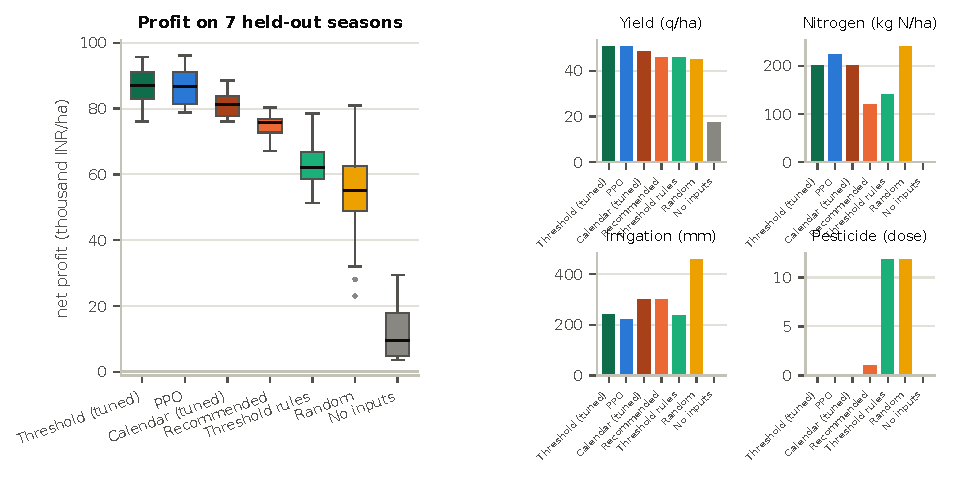
\includegraphics[width=0.96\columnwidth]{policy_comparison.pdf}
    \caption{Held-out Punjab performance (2017--2023): net profit boxplots (left) and mean yield and input usage (right). PPO gains $+11{,}935\text{ INR/ha}$ over the recommended calendar while saving $80\text{ mm}$ ($26.7\%$) of irrigation water.}
    \label{fig:policy_comp}
\end{figure}

\begin{figure}[t]
    \centering
    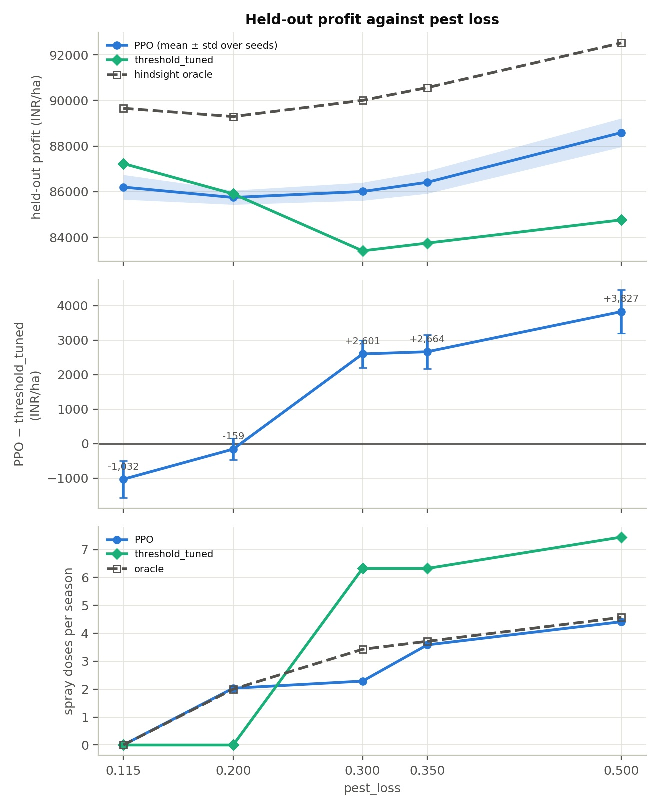
\includegraphics[height=3.35cm,keepaspectratio]{pest_sweep.pdf}\hfill
    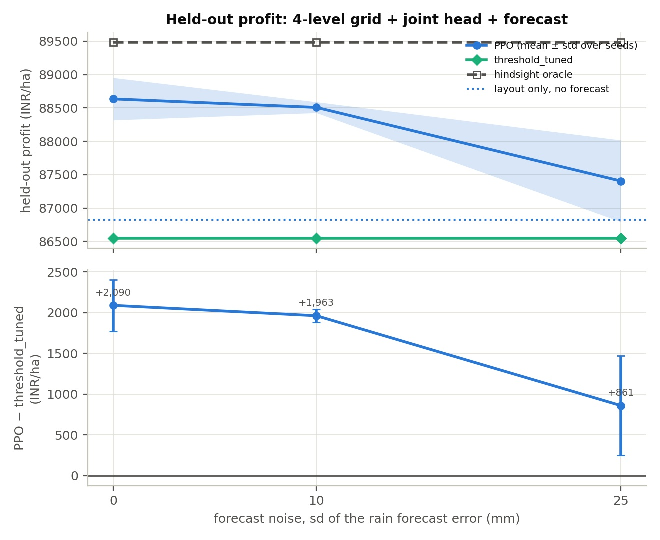
\includegraphics[height=3.35cm,keepaspectratio]{layout_forecast_sweep.pdf}
    \caption{\textbf{Left:} Across pest severity $L_p \in [0.115, 0.50]$, PPO beats the retuned threshold rule in 5/5 seeds for $L_p \ge 0.30$ ($+2.6\text{k}$ to $+3.8\text{k INR/ha}$) via selective spraying. \textbf{Right:} Combining a 4-level water grid + joint $N\times W$ head with a $10\text{ mm}$-error rain forecast reaches $88{,}508 \pm 81\text{ INR/ha}$ ($98.9\%$ of oracle).}
    \label{fig:sweeps}
\end{figure}

\section{Results \& Key Findings}
Table~\ref{tab:results} and Figures~\ref{fig:policy_comp}--\ref{fig:sweeps} summarise our findings across 12 systematic studies:
\begin{itemize}
    \item \textbf{Gain Over Extension Advice \& Oracle Ceiling:} On held-out seasons, PPO ($86{,}584 \pm 153\text{ INR/ha}$) beats the standard Recommended Calendar ($74{,}649\text{ INR/ha}$) by $\mathbf{+11{,}935\text{ INR/ha}}$ ($\mathbf{+16.0\%}$) while cutting irrigation by $\mathbf{26.7\%}$ ($220$ vs.\ $300\text{ mm}$). Shapley attribution across all $2^4$ decision coalitions shows $62\%$ of this gain comes from adaptive water timing and $31\%$ from nitrogen splitting. In the base setting, the coordinate-tuned threshold rule already reaches $97.3\%$ of the Hindsight Oracle ($87{,}232$ vs.\ $89{,}654\text{ INR/ha}$), leaving minimal room without weather foresight. PPO also outperforms Branching DQN ($83{,}617$) and CEM ($84{,}178$), while critic-free \textbf{GRPO} matches PPO ($86{,}223$) with $6\%$ faster training.
    \item \textbf{Selective Pest Control Under High Pest Severity:} At the aggregate calibration ($L_p = 0.115$), spraying does not pay off. When pest losses are significant ($L_p \ge 0.30$, Figure~\ref{fig:sweeps} left), \textbf{PPO beats the retuned threshold rule in all 5 seeds by $+2{,}601$ to $+3{,}827\text{ INR/ha}$}: PPO learns resistance-aware selective spraying ($3.6\text{ doses}$ at $L_p=0.35$, matching the oracle's $3.7$), whereas the reactive rule over-sprays ($6.3\text{ doses}$).
    \item \textbf{Rain Forecasts \& Joint Action Layout:} Oracle decomposition shows future weather knowledge is worth $+5{,}367\text{ INR/ha}$ vs.\ $+188\text{ INR/ha}$ for price knowledge. Adding a realistic next-fortnight rain forecast ($\sigma_R = 10\text{ mm}$) with a 4-level water grid and joint $N\times W$ head (Figure~\ref{fig:sweeps} right) lifts PPO to $\mathbf{88{,}508 \pm 81\text{ INR/ha}}$ ($\mathbf{98.9\%}$ of oracle), beating the tuned rule across all 5 seeds by $\mathbf{+1{,}963\text{ INR/ha}}$.
    \item \textbf{Zero-Shot Cross-State Transfer:} Transferred zero-shot from Punjab to \textbf{Haryana}, PPO achieves $\mathbf{74{,}303 \pm 463\text{ INR/ha}}$ ($96.2\%$ of Haryana oracle), outperforming the Haryana-tuned threshold rule ($73{,}831\text{ INR/ha}$) without retraining and remaining robust under $+2^\circ\text{C}$ and $-20\%$ rainfall stress tests.
\end{itemize}

\section{Conclusion}
\textbf{FarmRL} demonstrates that RL agents (PPO and critic-free GRPO) learn agro-economically sound policies that save water, avoid resistance-inducing over-spraying, and surpass tuned heuristic rules when pest pressure is nontrivial or short-range weather forecasts are available. The project includes an interactive 7-page Streamlit decision-support dashboard.

\vspace{2pt}
\noindent{\footnotesize\textbf{References}}\\[1pt]
{\scriptsize
[1] CACP, \textit{Price Policy for Rabi Crops: RMS 2027--28 (Annex Table 5.6a: Wheat Cost, Punjab \& Haryana)}, Govt.\ of India, 2026. \quad
[2] ICRISAT, TCI Cornell, \& IFPRI, \textit{District-Level Database for Indian Agriculture (1966--2017)}. \quad
[3] J.~Doorenbos \& A.~H.~Kassam, \textit{Yield Response to Water}, FAO Paper 33, 1979; P.~Steduto et al., \textit{AquaCrop}, FAO Paper 66, 2012. \quad
[4] M.~Rodell et al., ``Satellite-based estimates of groundwater depletion in India,'' \textit{Nature}, 460:999--1002, 2009. \quad
[5] J.~Schulman et al., ``Proximal Policy Optimization Algorithms,'' \textit{arXiv:1707.06347}, 2017; Z.~Shao et al., ``DeepSeekMath (GRPO),'' \textit{arXiv:2402.03300}, 2024.\par
}

\end{document}
